%% fig_frontier.tex   (generated by make_frontier.py; do not edit by hand)
%% The rule set of the closure theorem with the rules of the literature, as a hypergraph, and the five minimal sufficient sets, computed.
\documentclass[tikz,border=6pt]{standalone}
\usepackage{amsmath,amssymb}
\usetikzlibrary{arrows.meta,calc,decorations.pathreplacing,patterns}
%% palette.tex -- shared colour definitions for the figures
\definecolor{PInk}{RGB}{26,32,44}
\definecolor{PBlue}{RGB}{37,82,139}
\definecolor{PTeal}{RGB}{23,127,125}
\definecolor{POchre}{RGB}{193,138,44}
\definecolor{PClay}{RGB}{178,74,58}
\definecolor{PSlate}{RGB}{108,122,137}
\definecolor{PViolet}{RGB}{110,86,150}
\definecolor{WBlue}{RGB}{223,234,246}
\definecolor{WTeal}{RGB}{220,238,236}
\definecolor{WOchre}{RGB}{250,240,218}
\definecolor{WClay}{RGB}{247,229,224}
\definecolor{WSlate}{RGB}{238,241,244}
\definecolor{PMag}{RGB}{158,58,110}
\definecolor{PGrass}{RGB}{62,124,66}
\definecolor{PAmber}{RGB}{214,112,38}
\definecolor{PIndigo}{RGB}{58,64,140}
\definecolor{PRule}{RGB}{176,186,197}

%% shared macros so the standalone figures match the paper
\providecommand{\QQ}{\mathbb{Q}}
\providecommand{\ZZ}{\mathbb{Z}}
\providecommand{\RR}{\mathbb{R}}
\providecommand{\CC}{\mathbb{C}}
\providecommand{\PP}{\mathbb{P}}
\providecommand{\Kx}{K^{\times}}
\providecommand{\HW}{W}
\providecommand{\Nm}{\mathrm{N}}
\providecommand{\Hdg}{\mathrm{Hdg}}
\providecommand{\NS}{\mathrm{NS}}
\providecommand{\cA}{\mathcal{A}}
\providecommand{\cD}{\mathcal{D}}
\providecommand{\cF}{\mathcal{F}}
\providecommand{\cP}{\mathcal{P}}
\providecommand{\cO}{\mathcal{O}}
\providecommand{\cQ}{\mathcal{Q}}
\providecommand{\bbar}[1]{\overline{#1}}
\providecommand{\ch}{\operatorname{ch}}
\providecommand{\End}{\mathrm{End}}
\providecommand{\Ext}{\operatorname{Ext}}
\providecommand{\Supp}{\operatorname{Supp}}

\begin{document}
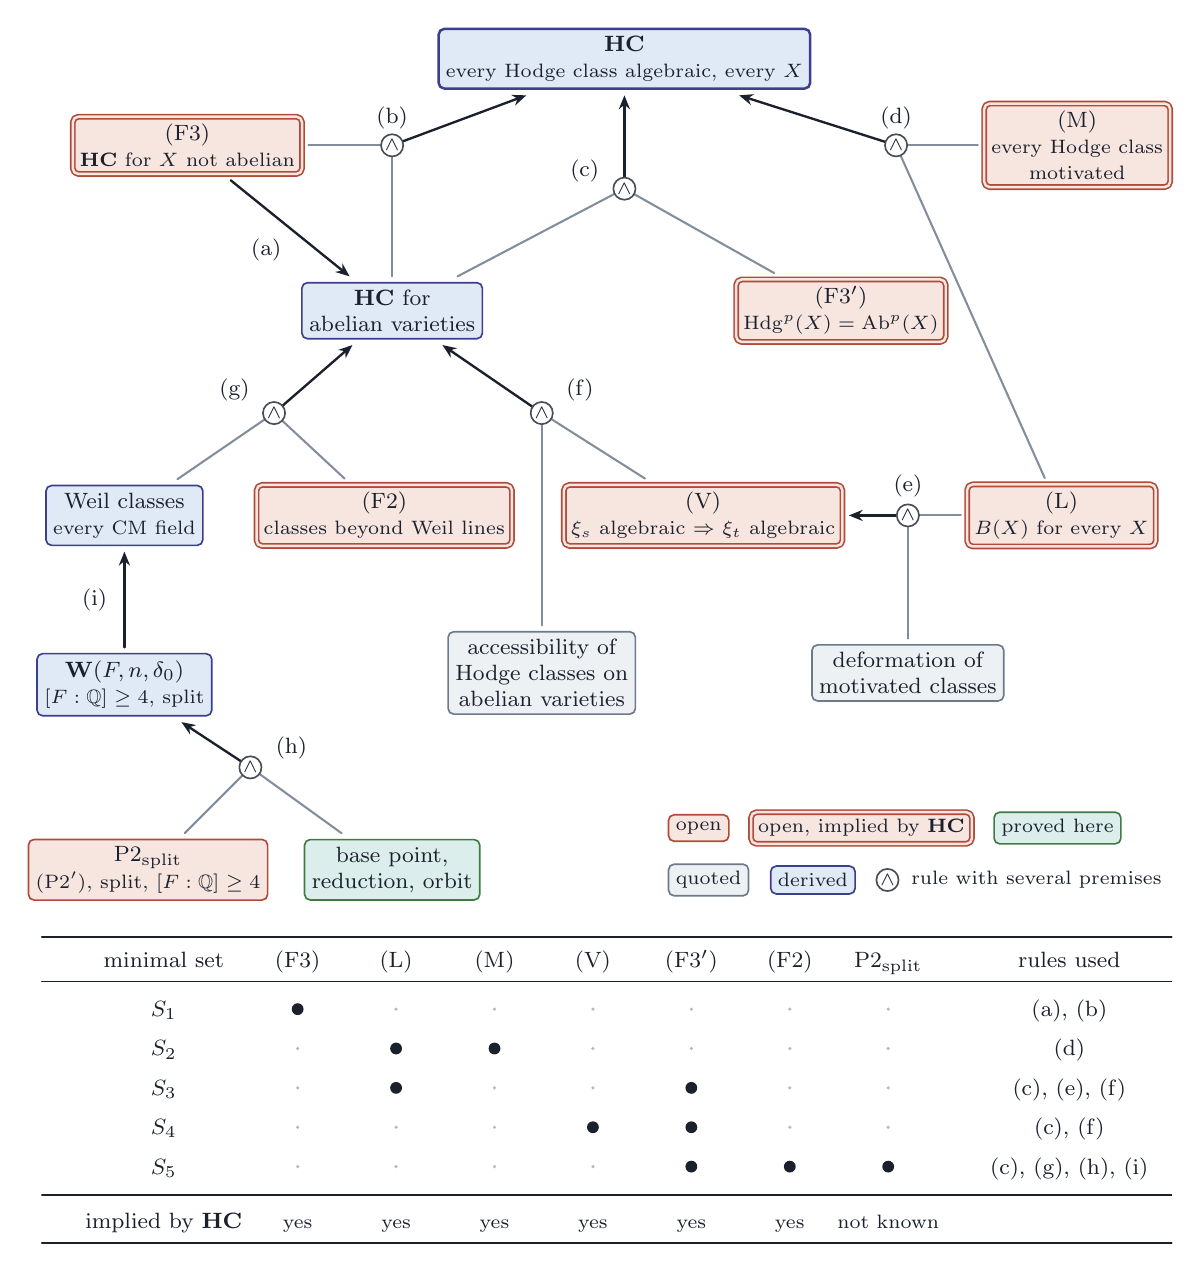
\begin{tikzpicture}[x=1cm,y=1cm,line join=round,line cap=round,
  font=\small,text=PInk]
  \draw[PInk,-{Stealth[length=5pt,width=4pt]},line width=0.85pt] (-5.000,7.506) -- (-3.490,6.286);
  \draw[PSlate!85,line width=0.75pt] (-2.950,6.286) -- (-2.950,7.813);
  \draw[PSlate!85,line width=0.75pt] (-4.014,7.950) -- (-3.087,7.950);
  \draw[PInk,-{Stealth[length=5pt,width=4pt]},line width=0.85pt] (-2.822,7.998) -- (-1.246,8.585);
  \draw[PSlate!85,line width=0.75pt] (-2.119,6.286) -- (-0.121,7.336);
  \draw[PSlate!85,line width=0.75pt] (1.902,6.328) -- (0.119,7.333);
  \draw[PInk,-{Stealth[length=5pt,width=4pt]},line width=0.85pt] (0.000,7.537) -- (0.000,8.585);
  \draw[PSlate!85,line width=0.75pt] (5.338,3.725) -- (3.506,7.825);
  \draw[PSlate!85,line width=0.75pt] (4.488,7.950) -- (3.587,7.950);
  \draw[PInk,-{Stealth[length=5pt,width=4pt]},line width=0.85pt] (3.319,7.992) -- (1.457,8.585);
  \draw[PSlate!85,line width=0.75pt] (4.272,3.250) -- (3.737,3.250);
  \draw[PSlate!85,line width=0.75pt] (3.600,1.686) -- (3.600,3.113);
  \draw[PInk,-{Stealth[length=5pt,width=4pt]},line width=0.85pt] (3.463,3.250) -- (2.850,3.250);
  \draw[PSlate!85,line width=0.75pt] (0.262,3.718) -- (-0.934,4.477);
  \draw[PSlate!85,line width=0.75pt] (-1.050,1.853) -- (-1.050,4.413);
  \draw[PInk,-{Stealth[length=5pt,width=4pt]},line width=0.85pt] (-1.163,4.627) -- (-2.312,5.414);
  \draw[PSlate!85,line width=0.75pt] (-5.677,3.710) -- (-4.563,4.473);
  \draw[PSlate!85,line width=0.75pt] (-3.554,3.718) -- (-4.350,4.457);
  \draw[PInk,-{Stealth[length=5pt,width=4pt]},line width=0.85pt] (-4.346,4.640) -- (-3.454,5.414);
  \draw[PSlate!85,line width=0.75pt] (-5.584,-0.784) -- (-4.847,-0.047);
  \draw[PSlate!85,line width=0.75pt] (-3.592,-0.786) -- (-4.639,-0.030);
  \draw[PInk,-{Stealth[length=5pt,width=4pt]},line width=0.85pt] (-4.865,0.125) -- (-5.626,0.625);
  \draw[PInk,-{Stealth[length=5pt,width=4pt]},line width=0.85pt] (-6.350,1.575) -- (-6.350,2.790);
  \node[draw=PIndigo,fill=WBlue,rounded corners=2pt,inner sep=2.6pt,line width=0.90pt,align=center,font=\footnotesize] at (0.000,9.050) {$\mathbf{HC}$\\{\scriptsize every Hodge class algebraic, every $X$}};
  \node[draw=PIndigo,fill=WBlue,rounded corners=2pt,inner sep=2.6pt,line width=0.60pt,align=center,font=\footnotesize] at (-2.950,5.850) {$\mathbf{HC}$ for\\abelian varieties};
  \node[draw=PClay,fill=WClay,rounded corners=2pt,inner sep=2.6pt,line width=0.60pt,align=center,font=\footnotesize,double=WClay,double distance=0.9pt] at (-5.550,7.950) {(F3)\\{\scriptsize $\mathbf{HC}$ for $X$ not abelian}};
  \node[draw=PClay,fill=WClay,rounded corners=2pt,inner sep=2.6pt,line width=0.60pt,align=center,font=\footnotesize,double=WClay,double distance=0.9pt] at (2.750,5.850) {(F3$'$)\\{\scriptsize $\mathrm{Hdg}^{p}(X)=\mathrm{Ab}^{p}(X)$}};
  \node[draw=PClay,fill=WClay,rounded corners=2pt,inner sep=2.6pt,line width=0.60pt,align=center,font=\footnotesize,double=WClay,double distance=0.9pt] at (5.750,7.950) {(M)\\{\scriptsize every Hodge class}\\{\scriptsize motivated}};
  \node[draw=PClay,fill=WClay,rounded corners=2pt,inner sep=2.6pt,line width=0.60pt,align=center,font=\footnotesize,double=WClay,double distance=0.9pt] at (5.550,3.250) {(L)\\{\scriptsize $B(X)$ for every $X$}};
  \node[draw=PClay,fill=WClay,rounded corners=2pt,inner sep=2.6pt,line width=0.60pt,align=center,font=\footnotesize,double=WClay,double distance=0.9pt] at (1.000,3.250) {(V)\\{\scriptsize $\xi_{s}$ algebraic $\Rightarrow$ $\xi_{t}$ algebraic}};
  \node[draw=PClay,fill=WClay,rounded corners=2pt,inner sep=2.6pt,line width=0.60pt,align=center,font=\footnotesize,double=WClay,double distance=0.9pt] at (-3.050,3.250) {(F2)\\{\scriptsize classes beyond Weil lines}};
  \node[draw=PIndigo,fill=WBlue,rounded corners=2pt,inner sep=2.6pt,line width=0.60pt,align=center,font=\footnotesize] at (-6.350,3.250) {Weil classes\\{\scriptsize every CM field}};
  \node[draw=PIndigo,fill=WBlue,rounded corners=2pt,inner sep=2.6pt,line width=0.60pt,align=center,font=\footnotesize] at (-6.350,1.100) {$\mathbf{W}(F,n,\delta_{0})$\\{\scriptsize $[F:\mathbb{Q}]\ge4$, split}};
  \node[draw=PClay,fill=WClay,rounded corners=2pt,inner sep=2.6pt,line width=0.60pt,align=center,font=\footnotesize] at (-6.050,-1.250) {$\mathrm{P2}_{\mathrm{split}}$\\{\scriptsize (P2$'$), split, $[F:\mathbb{Q}]\ge4$}};
  \node[draw=PGrass,fill=WTeal,rounded corners=2pt,inner sep=2.6pt,line width=0.60pt,align=center,font=\footnotesize] at (-2.950,-1.250) {base point,\\reduction, orbit};
  \node[draw=PSlate,fill=WSlate,rounded corners=2pt,inner sep=2.6pt,line width=0.60pt,align=center,font=\footnotesize] at (-1.050,1.250) {accessibility of\\Hodge classes on\\abelian varieties};
  \node[draw=PSlate,fill=WSlate,rounded corners=2pt,inner sep=2.6pt,line width=0.60pt,align=center,font=\footnotesize] at (3.600,1.250) {deformation of\\motivated classes};
  \node[circle,draw=PInk!80,fill=white,line width=0.6pt,inner sep=0.5pt,font=\scriptsize] at (-2.950,7.950) {$\wedge$};
  \node[circle,draw=PInk!80,fill=white,line width=0.6pt,inner sep=0.5pt,font=\scriptsize] at (0.000,7.400) {$\wedge$};
  \node[circle,draw=PInk!80,fill=white,line width=0.6pt,inner sep=0.5pt,font=\scriptsize] at (3.450,7.950) {$\wedge$};
  \node[circle,draw=PInk!80,fill=white,line width=0.6pt,inner sep=0.5pt,font=\scriptsize] at (3.600,3.250) {$\wedge$};
  \node[circle,draw=PInk!80,fill=white,line width=0.6pt,inner sep=0.5pt,font=\scriptsize] at (-1.050,4.550) {$\wedge$};
  \node[circle,draw=PInk!80,fill=white,line width=0.6pt,inner sep=0.5pt,font=\scriptsize] at (-4.450,4.550) {$\wedge$};
  \node[circle,draw=PInk!80,fill=white,line width=0.6pt,inner sep=0.5pt,font=\scriptsize] at (-4.750,0.050) {$\wedge$};
  \node[text=PInk,inner sep=1pt,align=center,font=\footnotesize] at (-4.550,6.620) {(a)};
  \node[text=PInk,inner sep=1pt,align=center,font=\footnotesize] at (-2.950,8.300) {(b)};
  \node[text=PInk,inner sep=1pt,align=center,font=\footnotesize,anchor=east] at (-0.280,7.620) {(c)};
  \node[text=PInk,inner sep=1pt,align=center,font=\footnotesize] at (3.450,8.300) {(d)};
  \node[text=PInk,inner sep=1pt,align=center,font=\footnotesize] at (3.600,3.620) {(e)};
  \node[text=PInk,inner sep=1pt,align=center,font=\footnotesize,anchor=west] at (-0.780,4.840) {(f)};
  \node[text=PInk,inner sep=1pt,align=center,font=\footnotesize,anchor=east] at (-4.720,4.840) {(g)};
  \node[text=PInk,inner sep=1pt,align=center,font=\footnotesize,anchor=west] at (-4.470,0.300) {(h)};
  \node[text=PInk,inner sep=1pt,align=center,font=\footnotesize,anchor=east] at (-6.530,2.180) {(i)};
  \node[draw=PClay,fill=WClay,rounded corners=2pt,inner sep=2.6pt,line width=0.60pt,align=center,font=\scriptsize,anchor=west] at (0.550,-0.720) {open};
  \node[draw=PClay,fill=WClay,rounded corners=2pt,inner sep=2.6pt,line width=0.60pt,align=center,font=\scriptsize,double=WClay,double distance=0.9pt,anchor=west] at (1.597,-0.720) {open, implied by $\mathbf{HC}$};
  \node[draw=PGrass,fill=WTeal,rounded corners=2pt,inner sep=2.6pt,line width=0.60pt,align=center,font=\scriptsize,anchor=west] at (4.684,-0.720) {proved here};
  \node[draw=PSlate,fill=WSlate,rounded corners=2pt,inner sep=2.6pt,line width=0.60pt,align=center,font=\scriptsize,anchor=west] at (0.550,-1.380) {quoted};
  \node[draw=PIndigo,fill=WBlue,rounded corners=2pt,inner sep=2.6pt,line width=0.60pt,align=center,font=\scriptsize,anchor=west] at (1.847,-1.380) {derived};
  \node[circle,draw=PInk!80,fill=white,line width=0.6pt,inner sep=0.5pt,font=\scriptsize] at (3.341,-1.380) {$\wedge$};
  \node[text=PInk,inner sep=1pt,align=center,font=\scriptsize,anchor=west] at (3.601,-1.380) {rule with several premises};
  \draw[PInk,line width=0.60pt] (-7.400,-2.100) -- (6.950,-2.100);
  \draw[PInk,line width=0.40pt] (-7.400,-2.670) -- (6.950,-2.670);
  \node[text=PInk,inner sep=1pt,align=center,font=\footnotesize,text height=1.7ex,text depth=0.45ex] at (-5.850,-2.400) {minimal set};
  \node[text=PInk,inner sep=1pt,align=center,font=\footnotesize,text height=1.7ex,text depth=0.45ex] at (-4.150,-2.400) {(F3)};
  \node[text=PInk,inner sep=1pt,align=center,font=\footnotesize,text height=1.7ex,text depth=0.45ex] at (-2.900,-2.400) {(L)};
  \node[text=PInk,inner sep=1pt,align=center,font=\footnotesize,text height=1.7ex,text depth=0.45ex] at (-1.650,-2.400) {(M)};
  \node[text=PInk,inner sep=1pt,align=center,font=\footnotesize,text height=1.7ex,text depth=0.45ex] at (-0.400,-2.400) {(V)};
  \node[text=PInk,inner sep=1pt,align=center,font=\footnotesize,text height=1.7ex,text depth=0.45ex] at (0.850,-2.400) {(F3$'$)};
  \node[text=PInk,inner sep=1pt,align=center,font=\footnotesize,text height=1.7ex,text depth=0.45ex] at (2.100,-2.400) {(F2)};
  \node[text=PInk,inner sep=1pt,align=center,font=\footnotesize,text height=1.7ex,text depth=0.45ex] at (3.350,-2.400) {$\mathrm{P2}_{\mathrm{split}}$};
  \node[text=PInk,inner sep=1pt,align=center,font=\footnotesize,text height=1.7ex,text depth=0.45ex] at (5.650,-2.400) {rules used};
  \node[text=PInk,inner sep=1pt,align=center,font=\footnotesize,text height=1.7ex,text depth=0.45ex] at (-5.850,-3.020) {$S_{1}$};
  \fill[PInk] (-4.150,-3.020) circle (0.075);
  \fill[PRule] (-2.900,-3.020) circle (0.022);
  \fill[PRule] (-1.650,-3.020) circle (0.022);
  \fill[PRule] (-0.400,-3.020) circle (0.022);
  \fill[PRule] (0.850,-3.020) circle (0.022);
  \fill[PRule] (2.100,-3.020) circle (0.022);
  \fill[PRule] (3.350,-3.020) circle (0.022);
  \node[text=PInk,inner sep=1pt,align=center,font=\footnotesize,text height=1.7ex,text depth=0.45ex] at (5.650,-3.020) {(a), (b)};
  \node[text=PInk,inner sep=1pt,align=center,font=\footnotesize,text height=1.7ex,text depth=0.45ex] at (-5.850,-3.520) {$S_{2}$};
  \fill[PRule] (-4.150,-3.520) circle (0.022);
  \fill[PInk] (-2.900,-3.520) circle (0.075);
  \fill[PInk] (-1.650,-3.520) circle (0.075);
  \fill[PRule] (-0.400,-3.520) circle (0.022);
  \fill[PRule] (0.850,-3.520) circle (0.022);
  \fill[PRule] (2.100,-3.520) circle (0.022);
  \fill[PRule] (3.350,-3.520) circle (0.022);
  \node[text=PInk,inner sep=1pt,align=center,font=\footnotesize,text height=1.7ex,text depth=0.45ex] at (5.650,-3.520) {(d)};
  \node[text=PInk,inner sep=1pt,align=center,font=\footnotesize,text height=1.7ex,text depth=0.45ex] at (-5.850,-4.020) {$S_{3}$};
  \fill[PRule] (-4.150,-4.020) circle (0.022);
  \fill[PInk] (-2.900,-4.020) circle (0.075);
  \fill[PRule] (-1.650,-4.020) circle (0.022);
  \fill[PRule] (-0.400,-4.020) circle (0.022);
  \fill[PInk] (0.850,-4.020) circle (0.075);
  \fill[PRule] (2.100,-4.020) circle (0.022);
  \fill[PRule] (3.350,-4.020) circle (0.022);
  \node[text=PInk,inner sep=1pt,align=center,font=\footnotesize,text height=1.7ex,text depth=0.45ex] at (5.650,-4.020) {(c), (e), (f)};
  \node[text=PInk,inner sep=1pt,align=center,font=\footnotesize,text height=1.7ex,text depth=0.45ex] at (-5.850,-4.520) {$S_{4}$};
  \fill[PRule] (-4.150,-4.520) circle (0.022);
  \fill[PRule] (-2.900,-4.520) circle (0.022);
  \fill[PRule] (-1.650,-4.520) circle (0.022);
  \fill[PInk] (-0.400,-4.520) circle (0.075);
  \fill[PInk] (0.850,-4.520) circle (0.075);
  \fill[PRule] (2.100,-4.520) circle (0.022);
  \fill[PRule] (3.350,-4.520) circle (0.022);
  \node[text=PInk,inner sep=1pt,align=center,font=\footnotesize,text height=1.7ex,text depth=0.45ex] at (5.650,-4.520) {(c), (f)};
  \node[text=PInk,inner sep=1pt,align=center,font=\footnotesize,text height=1.7ex,text depth=0.45ex] at (-5.850,-5.020) {$S_{5}$};
  \fill[PRule] (-4.150,-5.020) circle (0.022);
  \fill[PRule] (-2.900,-5.020) circle (0.022);
  \fill[PRule] (-1.650,-5.020) circle (0.022);
  \fill[PRule] (-0.400,-5.020) circle (0.022);
  \fill[PInk] (0.850,-5.020) circle (0.075);
  \fill[PInk] (2.100,-5.020) circle (0.075);
  \fill[PInk] (3.350,-5.020) circle (0.075);
  \node[text=PInk,inner sep=1pt,align=center,font=\footnotesize,text height=1.7ex,text depth=0.45ex] at (5.650,-5.020) {(c), (g), (h), (i)};
  \draw[PInk,line width=0.40pt] (-7.400,-5.380) -- (6.950,-5.380);
  \node[text=PInk,inner sep=1pt,align=center,font=\footnotesize,text height=1.7ex,text depth=0.45ex] at (-5.850,-5.710) {implied by $\mathbf{HC}$};
  \node[text=PInk,inner sep=1pt,align=center,font=\scriptsize,text height=1.7ex,text depth=0.45ex] at (-4.150,-5.710) {yes};
  \node[text=PInk,inner sep=1pt,align=center,font=\scriptsize,text height=1.7ex,text depth=0.45ex] at (-2.900,-5.710) {yes};
  \node[text=PInk,inner sep=1pt,align=center,font=\scriptsize,text height=1.7ex,text depth=0.45ex] at (-1.650,-5.710) {yes};
  \node[text=PInk,inner sep=1pt,align=center,font=\scriptsize,text height=1.7ex,text depth=0.45ex] at (-0.400,-5.710) {yes};
  \node[text=PInk,inner sep=1pt,align=center,font=\scriptsize,text height=1.7ex,text depth=0.45ex] at (0.850,-5.710) {yes};
  \node[text=PInk,inner sep=1pt,align=center,font=\scriptsize,text height=1.7ex,text depth=0.45ex] at (2.100,-5.710) {yes};
  \node[text=PInk,inner sep=1pt,align=center,font=\scriptsize,text height=1.7ex,text depth=0.45ex] at (3.350,-5.710) {not known};
  \draw[PInk,line width=0.60pt] (-7.400,-5.990) -- (6.950,-5.990);
\end{tikzpicture}
\end{document}
